\section{Evaluation}\label{section:evaluation}


\subsection{Vibration extraction experiment using simulated video}\label{subsection:eval:experiment1}

\begin{table}[tb]
  \centering
  \caption {Parameters to be evaluated}
  \label{table:bit_eval_parameter1}
  \begin{tabular}{|c|c|}
    %%\toprule
    \hline
    parameter   & value                \\ \hline \hline
    search window size & 11 \\\hline
    cell size   & 9          \\\hline
    %%BMFLCの通過周波数帯の分割数 & 16      \\\hline
    quantization bit width   & 2      \\\hline
     gain parameter of the BMFLC weight vector & $2^{-7}$ \\ \hline
    %%オプティカルフローの閾値   & 1.5                  \\ \hline
  \end{tabular}
\end{table}

%% 表\ref{table:bit_eval_parameter1}に、今回評価する振動抽出システムのパラメータと、
%% パラメータのデフォルト値を示す。

Table \ref{table:bit_eval_parameter1} shows the parameters of the vibration extraction system
to be evaluated in this study and the default values of the parameters.

%% 本研究では、評価指標にWMAPE(Weighted Mean Absolute Percentage Error)と相互相関係数の2つを用いた.
%% WMAPEは眞邉らの研究\cite{bib:Image-Based_Vibration_Extraction}で用いられた評価指標であり,
%% 出力値が真値に近いほど$0$に近い値を示し,出力値がすべて$0$である場合に1を示す.
%% 出力値を$x(k)$,真値を$y(k)$とすると,
%% 以下のように算出される:

Two evaluation indices, WMAPE (Weighted Mean Absolute Percentage Error) and cross-correlation coefficient, were used in this study.
WMAPE is the evaluation index used in the study by Manabe et al.
The closer the output value is to the true value,the closer the value is to $0$, and 1 is indicated when all output values are $0$.
Let $x(k)$ be the output value and $y(k)$ be the true value, and it is calculated as follows:


\begin{equation}
  \label{equ:WMAPE_origin}
  e_{\mathit{norm}} = \frac{\sum_{k} \left| x(k)-y(k) \right| }{\sum_{k} \left| y(k)  \right|}   
\end{equation}


%% 今回の評価では位相情報に着目した評価を行うため,$x(k)$,$y(k)$を独立に正規化するように変更した式を使用した:

In this evaluation,
we used the modified equation to normalize $x(k)$ and $y(k)$ independently in order to focus on the phase information:


\begin{equation}
  \label{equ:WMAPE}
  e_{\mathit{scale}} =  \sum_{k}  \left| \frac{\sum_{k} x(k)}{\sum_{k} |x(k)|}  - \frac{\sum_{k} y(k)}{\sum_{k} |y(k)|} \right|    
\end{equation}


%% また,相互相関係数とは$x(k)$,$y(k)$のそれぞれの分散$S_x$,$S_y$と共分散$S_{xy}$から,
%% で求められる評価指標である.
%% 正の相関が強いほど$1$に近い値を示し,負の相関が強いほど$-1$に近い値を示す評価関数である.
%% 相関がない場合は$0$に近い値を示す.
%% 相互相関係数は以下のように求められる。

The cross-correlation coefficient is an evaluation index calculated from the variance $S_x$, $S_y$
and covariance $S_{xy}$ of $x(k)$ and $y(k)$, respectively.
The stronger the positive correlation, the closer the value to $1$, and the stronger the negative correlation,
the closer the value to $1$. When there is no correlation,
the value is close to $0$. The cross-correlation coefficient is obtained as follows:

\begin{equation}
  \label{equ:cross-correlation}
  r= \frac{s_{xy}}{s_xs_y}
  =\frac{\frac{1}{n} \sum_{i=0}^{n}(x_i - \bar{x})(y_i - \bar{y})}
  {\sqrt{\frac{1}{n} \sum_{i=0}^{n}(x_i-\bar{x})^2}\sqrt{\frac{1}{n} \sum_{i=0}^{n}(y_i-\bar{y})^2}}    
\end{equation}



%% なお,適応推定フィルタであるBMFLCは適応するまでに一定の時間を要するため,$750$フレームのデータのうち,
%% $300$フレームから$750$フレームの出力値を評価対象とした.

Since the adaptive estimation filter, BMFLC, takes a certain amount of time to adapt,
the output values from $300$ to $750$ frames out of $750$ frames of data were the target of evaluation.


%% まずはじめに、オプティカルフローの探索ウインドウサイズを変化させた際の出力値の評価結果を表\ref{table_window_size}示す。
%% ウインドウサイズが大きくなるほどWMAPEの値は低下し,相互相関係数の値が上昇していることがわかる.
%% このことから,ウインドウサイズを大きくすることが抽出精度の向上に効果的であることが分かった.

First of all, the results of the evaluation of the output values when the optical flow search window size is
varied are shown in Table \ref{table:window_size}.
It can be seen that as the window size increases,
the value of WMAPE decreases and the value of the cross-correlation coefficient increases.
This indicates that increasing the window size is effective in improving the extraction accuracy.


\begin{table}[tb]
  \centering
  \caption{Evaluation results when search window size is varied}
  \label{table:window_size}
  \begin{tabular}{|c|c|c|}
    %%\toprule
    \hline
    search window size   & WMAPE &cross correlation  \\ \hline \hline
    9         &1.42930  &0.31552       \\ \hline
    11        &0.76671  &0.66365 \\ \hline
    13        &0.67171  &0.73732 \\ \hline
    15        &0.64146  &0.76056  \\ \hline
    17        &0.54591  &0.82015  \\ \hline
    19        &0.49598  &0.84790   \\ \hline
    21        &0.42631  &0.87880  \\ \hline
    23        &0.40533  &0.88938   \\ \hline
    25        &0.37493  &0.90636  \\ \hline
    27        &0.35800  &0.91632   \\ \hline
  \end{tabular}
\end{table}




%% 次に,セルサイズを変化させた場合の評価を行った.ウインドウサイズは先ほどの評価で最も抽出精度が高かった
%% 27を使用し,その他のパラメータはパラメータ群1の値に固定した.
%% 各セルサイズにおける評価結果を表\ref{table:cell_size}に示す.
%% ウインドウサイズ同様に,セルサイズが大きくなるほどWMAPEの値は低下し,相互相関係数の値が上昇していることがわかる.
%% このことから,セルサイズを大きくすることが抽出精度の向上に効果的であることが分かった.


Next, the evaluation was conducted for varying cell size.
The search window size was set to $27$, which had the highest extraction accuracy in the previous evaluation.
The evaluation results for each cell size are shown in Table \ref{table:cell_size}.
As with the search window size, it can be seen that as the cell size increases,
the value of WMAPE decreases and the value of the cross-correlation coefficient increases.
This indicates that increasing the cell size is effective in improving the extraction accuracy.


\begin{table}[tb]
 \centering
 \caption{Evaluation results when cell size is varied}
 \label{table:cell_size}
 \begin{tabular}{|c|c|c|}
   %%\toprule
   \hline
   cell size & WMAPE &cross correlation \\ \hline \hline
   9         &0.35799  &0.91632       \\ \hline
   11        &0.34619  &0.92174 \\ \hline
   13        &0.33681  &0.92742 \\ \hline
   15        &0.32301  &0.93433  \\ \hline
   17        &0.32081  &0.93625  \\ \hline
   19        &0.32086  &0.93686   \\ \hline
   21        &0.31727  &0.93987  \\ \hline
   23        &0.31078  &0.94436   \\ \hline
   25        &0.30074  &0.94905   \\ \hline
   27        &0.28922  &0.95342 \\ \hline
 \end{tabular}
\end{table}



%% 次に,BMFLCの適応ゲインパラメータを変化させた場合の評価を行った.
%% 各ゲインパラメータにおける評価結果を表\ref{table:gain}に示す.
%% ゲインパラメータを大きくすると,収束速度が向上する半面,安定性が損なわれ,WMAPEの値は大きく,相互相関係数の値は小さい.
%% また,ゲインパラメータを小さくすると安定性が向上する半面,収束速度が低下し,300フレームからの750フレームの評価では
%% 抽出精度が低下する傾向があることが分かった.


Next, we evaluated the BMFLC when the adaptive gain parameters were varied.
The evaluation results for each gain parameter are shown in Table \ref{table:gain}.
As the gain parameter is increased, the convergence speed increases, but stability is impaired,
and the WMAPE value is larger and the cross-correlation coefficient is smaller.
When the gain parameter is decreased, the stability improves, but the convergence speed decreases,
and the extraction accuracy tends to decrease for the evaluation of 750 frames from 300 frames.


\begin{table}[tb]
  \centering
  \caption{Evaluation results when gain parameter is varied}
  \label{table:gain}
  \begin{tabular}{|c|c|c|}
    %%\toprule
    \hline
    gain parameter   & WMAPE & cross correlation     \\ \hline \hline
    $2^{-3}$        &1.29598 &0.04524       \\ \hline
    $2^{-4}$        &1.36716  & -0.0142 \\ \hline
    $2^{-5}$        &0.97749  &0.53896 \\ \hline
    $2^{-6}$       &0.32301  &0.88169  \\ \hline
    $2^{-7}$        &0.28922  &0.95342  \\ \hline
    $2^{-8}$        &0.22523  &0.97019   \\ \hline
    $2^{-9}$        &0.22797  &0.968040  \\ \hline
    $2^{-10}$       &0.27036  &0.947585  \\ \hline
  \end{tabular}
\end{table}


%% 最後に、勾配方向の量子化ビット幅を変化させた際の出力値の評価を行った。
%% その他のパラメータについて、表\ref{table:quan_param}に示す2パターンのパラメータ群を用意し、
%% それぞれのパターンの量子化ビット幅を変更する。
%% 各パターンにおける評価結果を表\ref{table:quan}に示す。
%% パターン$1$においては量子化ビット幅を大きくするほど抽出精度が良くなっているが、
%% パターン$2$においては、量子化ビット幅を大きくするほど抽出精度が悪くなっていることがわかる。
%% この結果から、量子化ビット幅はその他のパラメータによって,適した値が変わることがわかった。


Finally, the output values were evaluated when the quantization bit width in the gradient direction was varied.
For the other parameters, we prepared a group of parameters for the two patterns shown in Table \ref{table:quan_param}
and changed the quantization bit width for each pattern.
The evaluation results for each pattern are shown in table\ref{table:quan_param}.
It can be seen that in pattern $1$,the extraction accuracy improves as the quantization bit width is increased,
while in pattern $2$, the extraction accuracy worsens as the quantization bit width is increased.
This result indicates that the appropriate value of the quantization bit width varies depending on other parameters.


\begin{table}[tb]
  \centering
  \caption {Parameters to be evaluated}
  \label{table:quan_param}
  \begin{tabular}{|c|c|c|}
    %%\toprule
    \hline
    parameter                & pattern 1 & pattern2 \\ \hline \hline
    search window size       &   9       &   19 \\\hline
    cell size                &   9       &   19 \\\hline
    gain parameter of the BMFLC weight vector & $2^{-7}$ & $2^{-7}$  \\ \hline
  \end{tabular}
\end{table}



\begin{table}[tb]
  \centering
  \caption{Evaluation results when quantization bit width}
  \label{table:quan}
  \begin{tabular}{|c|c|c|c|}
    %%\toprule
    \hline
    pattern & quantization bit width   & WMAPE & cross correlation     \\ \hline \hline
    1       &  1         &1.98376   &  0.05763       \\ \hline
    1       &  2         &1.42930   &  0.31552    \\ \hline
    1       &  3         &1.20372   &  0.36329 \\ \hline
    2       &  1         &0.39431   &  0.89721  \\ \hline
    2       &  2         &0.47363   &  0.85405  \\ \hline
    2       &  3         &0.48867   &  0.84429   \\ \hline
  \end{tabular}
\end{table}






\subsection{Vibration experiments using a vibratory apparatus}\label{subsection:eval:add_experiment}

\begin{table}[tb]
  \centering
  \caption{Parameters of the system during the vibration experiment}
  \label{bit_table:vibration_parameter}
  \begin{tabular}{|c|c|}
    %%\toprule
    \hline
    parameter   & value                \\ \hline \hline
    search window size & 27 \\\hline
    cell size   & 27          \\\hline
    %%BMFLCの通過周波数帯の分割数 & 16      \\\hline
    quantization bit width   & 2      \\\hline
    gain parameter of the BMFLC weight vector & $2^{-7}$ \\ \hline
    %%オプティカルフローの閾値   & 1.5                  \\ \hline
  \end{tabular}
\end{table}


%% 表\ref{bit_table:vibration_parameter}に加振実験を行った際の振動抽出FPGAシステムのパラメータを示す.
%% 図\ref{figure:supp_eval:vibration_test_result},図\ref{figure:supp_eval:vibration_test_result_fft}に
%% 加振実験の結果を示す.
%% 図\ref{figure:supp_eval:vibration_test_result}は,縦軸が移動位置,横軸が時間の波形であり,約$1.3 \sim 4.5$秒間
%% にズームした図である.オレンジ線がインタフェースが出力した値,青線がVIPERで測定した加振実験の結果である.
%% また,図\ref{figure:supp_eval:vibration_test_result_fft}は図\ref{figure:supp_eval:vibration_test_result}の結果の
%% 振幅スペクトルである.

%% 図\ref{figure:supp_eval:vibration_test_result},
%% 図\ref{figure:supp_eval:vibration_test_result_fft}の通り,
%% 逆位相波発生装置の加振結果には,インタフェースが出力した
%% 振動データに含まれない振動成分が含まれていることがわかった.
%% そのため,逆位相波発生装置が振動抽出FPGAシステムの振動データを
%% 正確に加振できているとは言えない結果となった.


Table \ref{bit_table:vibration_parameter} shows the parameters of the vibration extraction system during the shaker experiments.
Figure\ref{figure:supp_eval:vibration_test_result} and Figure\ref{figure:supp_eval:vibration_test_result_fft} show
the results of the shaking experiment. Figure\ref{figure:supp_eval:vibration_test_result} shows the waveform with
the vertical axis representing the moving position and the horizontal axis representing time,
zoomed in for about $1.3 \sim 4.5$ seconds.
The figure is zoomed to about $1.3 \sim 4.5$s.
The orange line is the value output by the interface.
The orange line is the value output by the interface, and the blue line is the result of the vibration experiment measured by VIPER.
Figure\ref{figure:supp_eval:vibration_test_result_fft} is the amplitude spectrum of the result of Figure \ref{figure:supp_eval:vibration_test_result}.
shown in Figures \ref{figure:supp_eval:vibration_test_result} and \ref{figure:supp_eval:vibration_test_result_fft},
the vibration results of the antiphase vibratory apparatus include vibration components that are not included
in the vibration data output by the interface.
Therefore, it cannot be said that the antiphase vibratory apparatus accurately excites the
vibration data of the vibration extraction FPGA system.



\begin{figure}[tb]
  \centering
  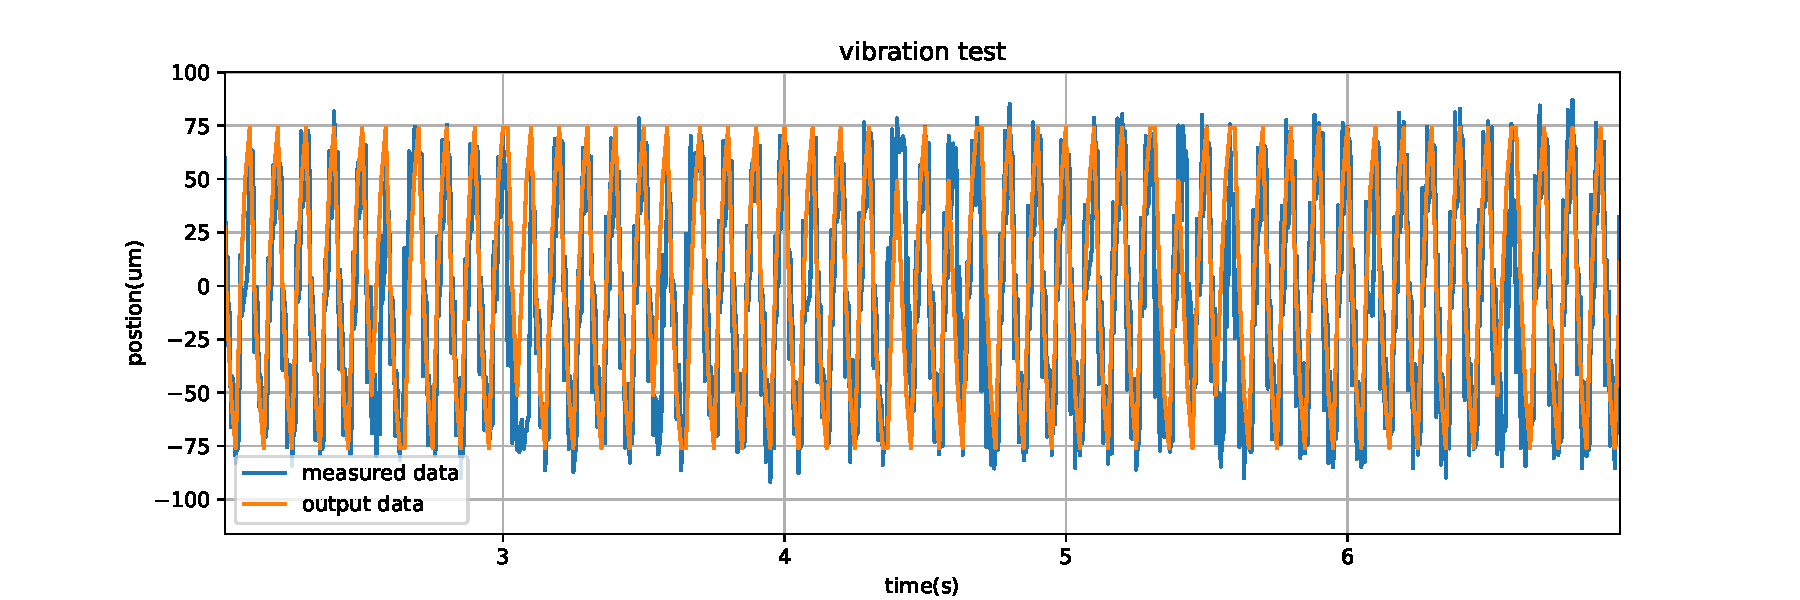
\includegraphics[width = 10cm,pagebox=cropbox,clip]{img/Supdevice_result.pdf}
  \caption{result:vibration experiment}
  \label{figure:supp_eval:vibration_test_result}
\end{figure}

\begin{figure}[tb]
  \centering
  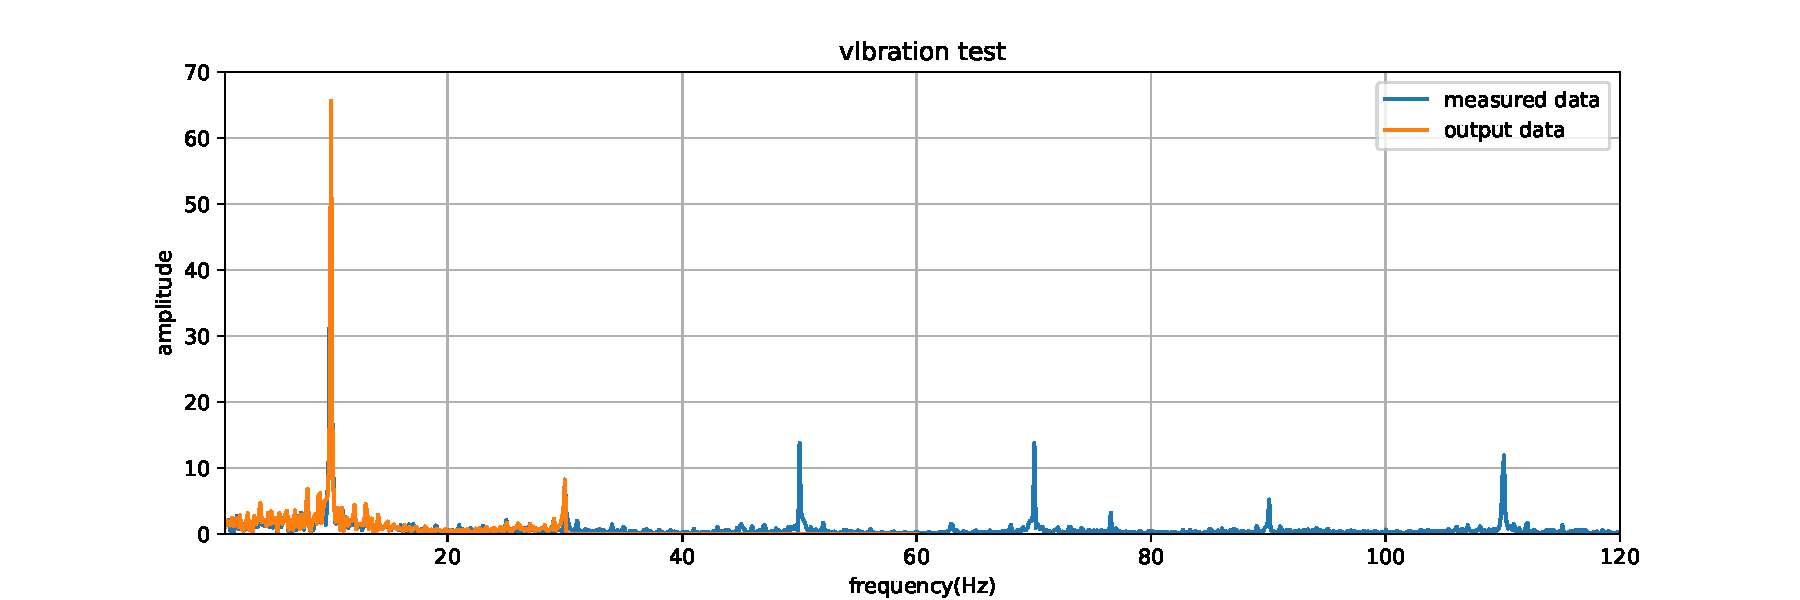
\includegraphics[width = 10cm,pagebox=cropbox,clip]{img/Supdevice_result_fft.pdf}
  \caption{spectrum:vibration experiment}
  \label{figure:supp_eval:vibration_test_result_fft}
\end{figure}








\subsection{ Tremor suppression experiment using a tremor reproduction device}\label{subsection:eval:suppression_experiment}

%% 抑制実験の結果を図\ref{figure:saupp_eval:10Hz_supp}に示す.
%% また,抑制結果の振幅スペクトルを図\ref{figure:saupp_eval:10Hz_supp_fft}に示す.
%% 図\ref{figure:saupp_eval:10Hz_supp}からわかるように,振幅の低下と
%% 増大が周期的に現れていることがわかる.


The results of the suppression experiment are shown in Figure\ref{figure:saupp_eval:10Hz_supp}.
The amplitude spectrum of the suppression results is shown in Figure\ref{figure:saupp_eval:10Hz_supp_fft}.
As can be seen from Figure\ref{figure:saupp_eval:10Hz_supp},
the amplitude decreases and increases periodically.


  \begin{figure}[tb]
    \centering
    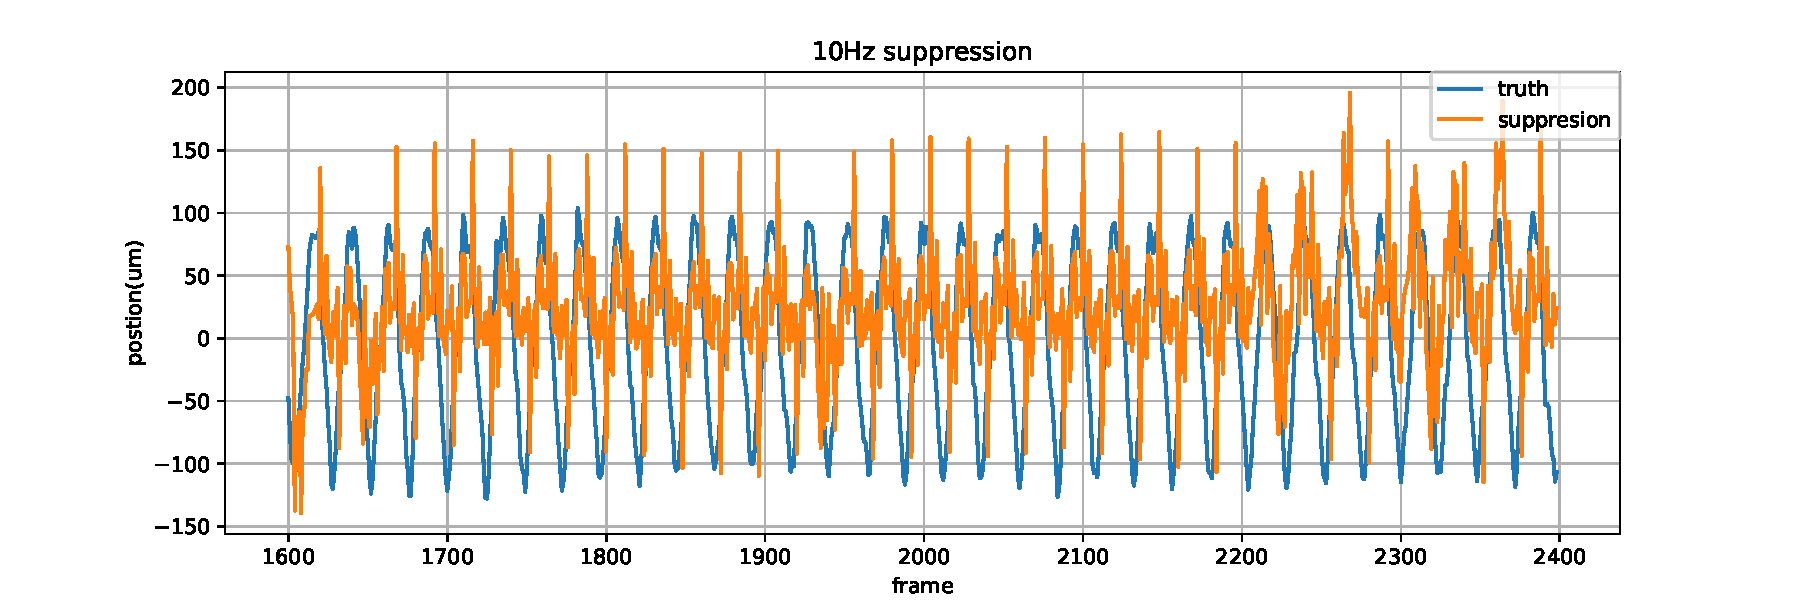
\includegraphics[width = 10cm,pagebox=cropbox,clip]{img/suppression_result.pdf}
    \caption{result:tremor suppression experiment}
    \label{figure:saupp_eval:10Hz_supp}
  \end{figure}
  
  \begin{figure}[tb]
    \centering
    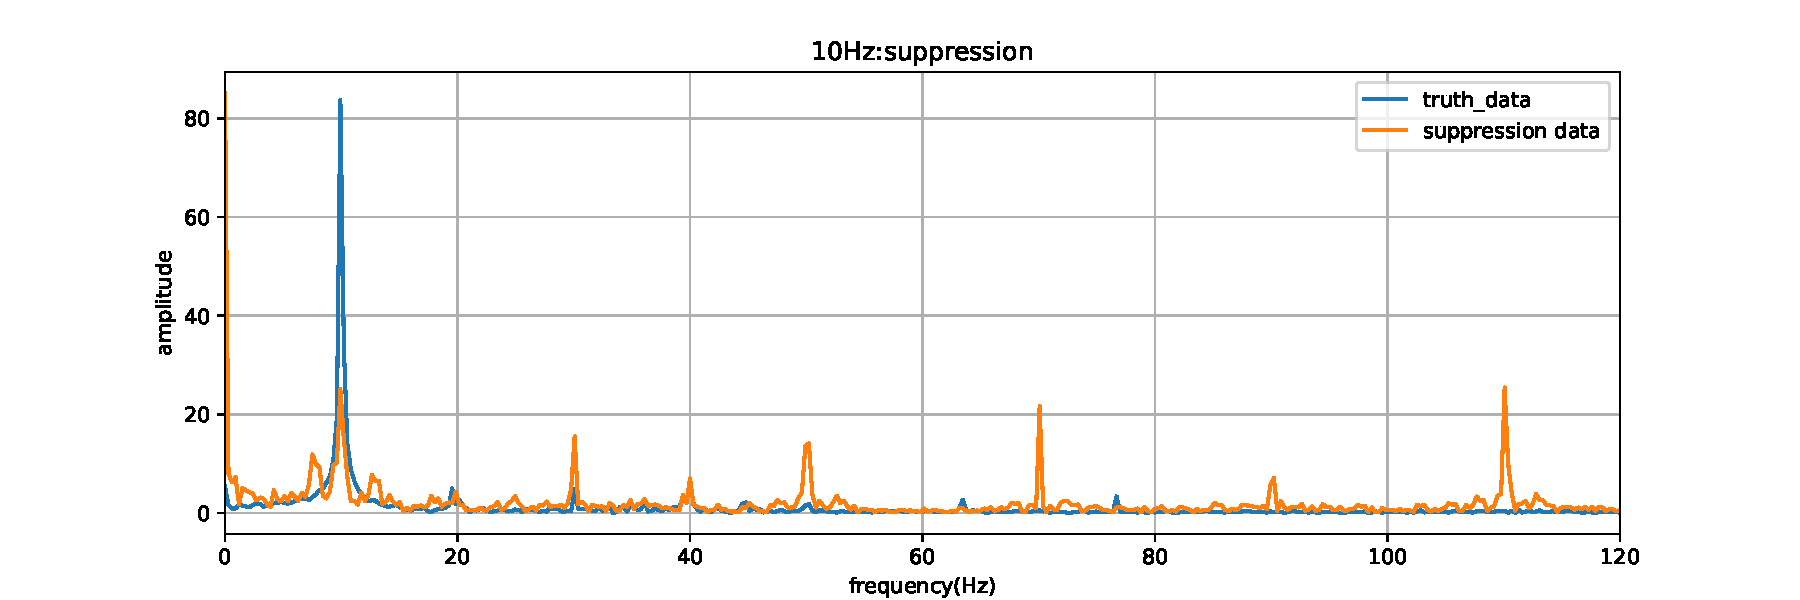
\includegraphics[width = 10cm,pagebox=cropbox,clip]{img/suppression_result_fft.pdf}
    \caption{spectrum:tremor suppression experiment}
    \label{figure:saupp_eval:10Hz_supp_fft}
  \end{figure}
